%\addcontentsline{toc}{part}{Exercices}

\chapter{Dualité onde-corpuscule}

\textit{Sources} : Schaum, chapitre 1 ; Cohen-Tannoudji, complément I-K.

\paragraph{Exercice 1} \textit{L'effet photoélectrique.} \\
L'effet photoélectrique fut découvert par hasard par Heinrich Hertz en 1887, alors qu'il s'employait à créer un appareil capable de générer des ondes électromagnétiques. Il s'agit d'un des nombreux processus physiques permettant d'extraire des électrons d'une surface métallique. Ses propriétés furent étudiées en plus grand détails quelques années plus tard par Philipp Lenard au moyen du dispositif expérimental que voici.
 
\begin{figure}[h!]
\begin{center}
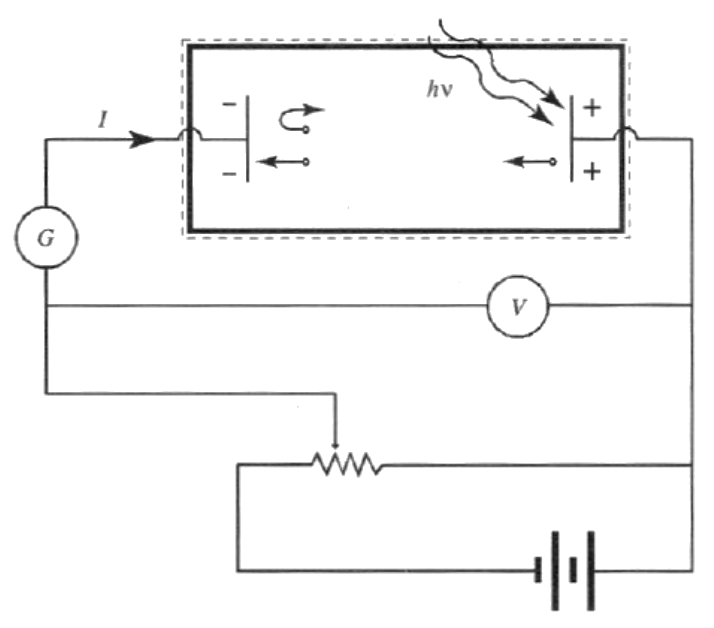
\includegraphics[width=0.45\textwidth]{Pictures/Photoelectrique.PNG}
\end{center}
\caption{\textit{Schéma de l'appareil destiné à l'étude de l'effet photoélectrique.}}
\end{figure}

On se munit d'un tube à vide contenant une électrode en Zinc. Cette dernière est éclairée par un rayon lumineux monochromatique de fréquence $\nu$. On constate que cette irradiation provoque l'émission d'électrons par la plaque de Zinc, lesquels seront collectés par une autre électrode située à l'autre extrémité du tube à vide. Les deux électrodes sont reliées entre elles par un circuit électrique muni d'un générateur de tension réglable, d'un volt-mètre et d'un ampère-mètre. 
\begin{enumerate}
\item La lumière fournit une quantité d'énergie $E$ à un électron de la plaque émettrice, convertie en travail d'extraction $W$ et énergie cinétique de l'électron libéré : $E = W + \frac{1}{2}mv^2$.
\item Lorsque l'électron est collecté par la seconde électrode, une différence de potentiel s'établit entre les deux électrodes du ``condensateur'' enfermé dans le tube à vide, ce qui crée un courant dans le circuit extérieur, mesuré par l'ampère-mètre. 
\item En outre, un générateur de tension réglable est introduit dans le circuit. Il fournit une différence de potentiel $V$ entre l'électrode émettrice et l'électrode réceptrice, appelée \textit{potentiel retardateur}.
\end{enumerate} 
$ $\\

\pagebreak

\textbf{Questions} \\
\begin{enumerate}
\item Expliquez le fait expérimental suivant : 
\begin{center}
\textit{Pour un signal lumineux de fréquence et d'intensité donnée, l'intensité du courant diminue lorsqu'on augmente le potentiel retardateur, jusqu'à atteindre 0 pour une valeur $V=V_0$ appelé \emph{potentiel d'arrêt}}.
\end{center}
Quelle quantité dynamique la mesure de $V_0$ permet-elle de déterminer ?
\item Voici un second fait expérimental.
\begin{center}
\textit{Pour une surface donnée, $V_0$ dépend de la couleur du rayonnement mais \emph{pas} de son intensité. Pour chaque métal, il existe une fréquence de seuil $\nu_s$ en-dessous de laquelle aucun courant n'est observé, et ce, quelle que soit l'intensité du rayon de lumière.}
\end{center}
Est-ce un résultat attendu, considérant la théorie ondulatoire de la lumière ?
\item Dans l'hypothèse d'Einstein, la lumière se comporte comme un flux de paquets insécables d'énergie $E=h\nu$, appelés \textit{photons}. Interprétez le résultat expérimental cité à la question précédente à la lumière de cette hypothèse.
Établissez et représentez graphiquement la relation entre $V_0$ et $\nu$, et expliquez pourquoi $\nu_s$ ne dépend que du métal employé.
\item Expérimentalement, on remarque aussi que le courant s'établit presque instantanément lorsqu'on allume le faisceau de lumière, même à très faible intensité lumineuse. Cela vous paraît-il plausible dans l'optique de la théorie ondulatoire ? Et avec l'hypothèse de quantification d'Einstein ?
\item Pour rendre plus précise la réponse à la question précédente, effectuons le petit calcul que voici. Supposons que nous éclairions (en incidence normale) une surface métallique avec une lumière d'intensité $10^{-10}\, W/m^2$. La distance moyenne entre 2 atomes du métal est de $3 \,\mathring{A}$, et chaque atome dispose d'un électron libre. L'énergie de liaison de cet électron est évaluée à $5 \, eV$. Supposons encore que la lumière est distribuée uniformément sur la surface, et que l'énergie est parfaitement absorbée par les électrons en surface. Si la radiation incidente est traitée classiquement (théorie ondulatoire), calculez le temps moyen d'irradiation qui devra s'écouler avant qu'un électron ne gagne assez d'énergie pour pouvoir être éjecté comme photo-électron ?
\end{enumerate}

\paragraph{Exercice 2} \textit{L'effet Compton.} \\
Selon la théorie quantique, un rayonnement électromagnétique monochromatique de fréquence $\nu$ peut être considéré comme un flux de photons, assimilables sous maints aspects à des particules, chacun possédant une quantité indivisible d'énergie $E=h\nu$ et une quantité de mouvement satisfaisant à la loi de De Broglie, $p = h\nu/c = h/\lambda$ ($c$ est la vitesse de la lumière dans le vide, et $\lambda$ la longueur d'onde du rayonnement). La diffusion de la lumière devient alors un problème de collision des photons avec des particules matérielles. 

\begin{figure}[h!]
\begin{center}
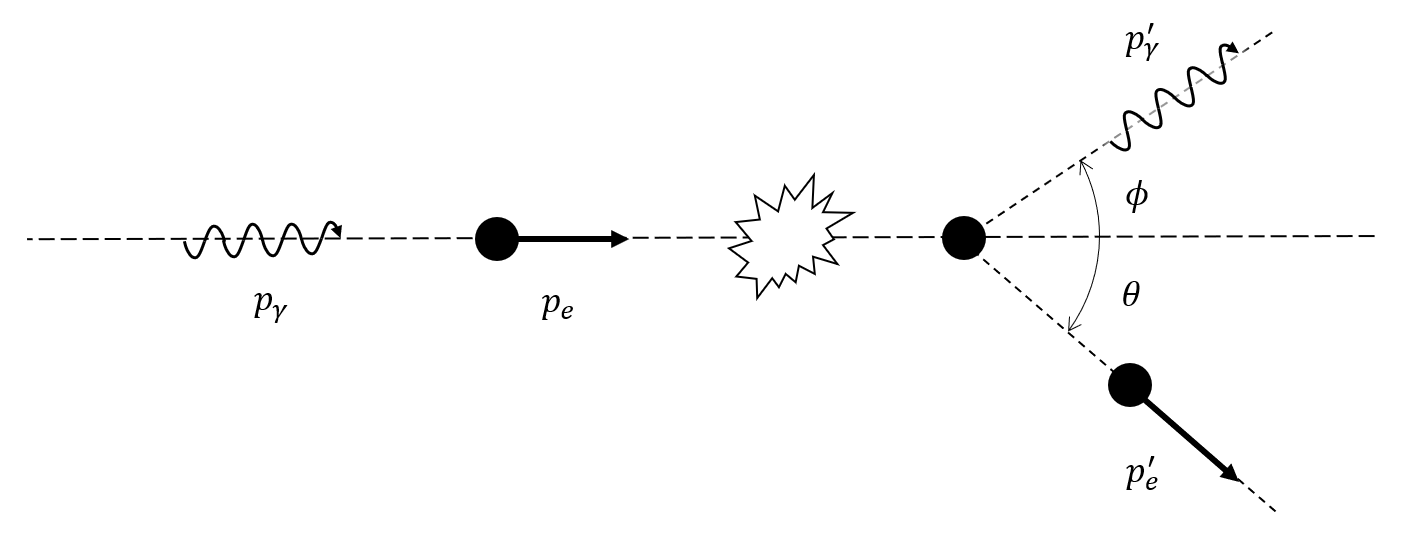
\includegraphics[width=0.75\textwidth]{Pictures/Compton.PNG}
\end{center}
\caption{\textit{Représentation schématique de la diffusion Compton.}}
\end{figure}

Supposons qu'un photon, d'impulsion $p_\gamma$, se déplace le long de l'axe $\vec{Ox}$, et rencontre un électron de quantité de mouvement $p_e$. Pour des raisons de simplicité, nous considérons que ce vecteur est aligné avec la direction de propagation du photon. Après collision, la trajectoire et la fréquence du photon sont modifiées (voir schéma pour la définition des diverses quantités). Ce phénomène, observé par Arthur Compton en 1923, acheva de convaincre les derniers sceptiques à l'égard du modèle corpusculaire de la lumière.
\begin{enumerate}
\item Écrivez la conservation de la quantité de mouvement et calculez $p'_e$.
\item Écrivez la conservation de l'énergie (relativiste) et montrez que l'énergie du photon diffusé est donnée par
\begin{equation}
E'_\gamma = \frac{E_\gamma (p_e c - E_e)}{E_\gamma (\cos\phi-1) + p_e c \cos\phi - E_e}.
\end{equation}
\item Établissez le déplacement en longueur d'onde du photon $\Delta\lambda_\gamma = \lambda_\gamma'-\lambda_\gamma$. 
\item On considère désormais que l'électron est initialement au repos. Évaluez la longueur d'onde de Compton de l'électron (pour laquelle le photon est diffusé dans la direction normale à la ligne d'incidence). Quel est le gain relatif en longueur d'onde pour de la lumière visible ($\lambda \approx 4000 \, \mathring{A}$) ? Pour du rayonnement X ($\lambda \approx 1 \, \mathring{A}$) ?
\item Calculez l'énergie transférée à l'électron en fonction de l'angle de déviation du photon. Discutez les deux régimes $E_\gamma \ll m_e c^2$ (\textit{diffusion de Thomson}) et $E_\gamma \gg m_e c^2$.
\item Montrez que $(1 + \sigma) \tan \theta = \cot (\phi/2)$ pour une constante $\sigma$ que l'on déterminera. Discutez les deux cas extrêmes $\phi=0$ et $\phi=\pi$. Pouviez-vous prévoir ce type de comportement ?
\end{enumerate}

\paragraph{Exercice 3} \textit{La diffusion de fullerènes.} \\
Les \textit{fullerènes} sont des nanoparticules formées d'un complexe de 60 atomes de carbone ($C_{60}$), et dont le nom fait référence à l'illustre architecte Buckminster Fuller (1895-1983). En 2000, elles furent utilisées par des chercheurs autrichiens pour réaliser une expérience de diffraction quantique, illustrant de manière prodigieuse la dualité onde-corpuscule pour des molécules plus complexes et massives que de simples particules élémentaires. 

\begin{figure}[h!]
\begin{center}
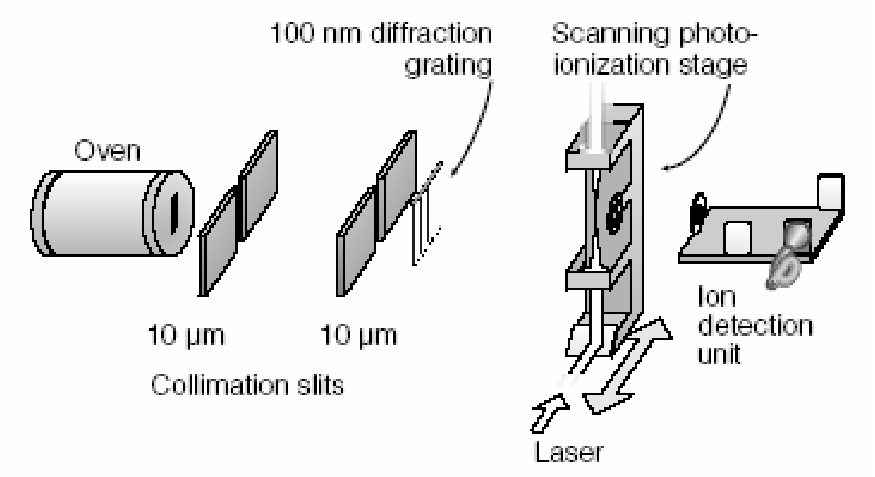
\includegraphics[width=0.55\textwidth]{Pictures/Fullerenes.PNG}
\end{center}
\caption{\textit{Dispositif expérimental. Source: [Nature \textbf{401} (2000) 691].}}
\end{figure}

\begin{enumerate}
\item Les fullerènes étaient émises par une petite ouverture dans un four chauffé à $1000 \, K$. Quelle est leur énergie cinétique, leur impulsion, leur longueur d'onde de De Broglie ?
\item Après collimation, les nanoparticules passaient à travers un réseau dont les fentes étaient espacées de $100\, nm$. Elles se propageaient ensuite sur $1.25 \, m$ avant d'être détectées. Estimez l'interfrange attendu sur la figure de diffraction. La détection s'opérait par focalisation d'un faisceau de lumière visible intense qui ionisaient les fullerènes. Les ions obtenus étaient accélérés par un champ électrique et détectés. L'interfrange est-elle compatible avec la méthode de détection utilisée ?
\end{enumerate}
Voici les résultats de l'expérience. Les deux figures reprennent les coups enregistrés dans le détecteur en fonction de la position de celui-ci, en haut, en présence du réseau, en bas, en l'absence du réseau. On remarque clairement la présence d'interférences, et leur position s'ajuste assez fidèlement aux courbes lisses en surimpression, qui représentent la figure de diffraction attendue dans une théorie purement ondulatoire de la propagation. Ceci nous indique que le comportement collectif des nanoparticules est sans conteste ondulatoire.

\begin{figure}[h!]
\begin{center}
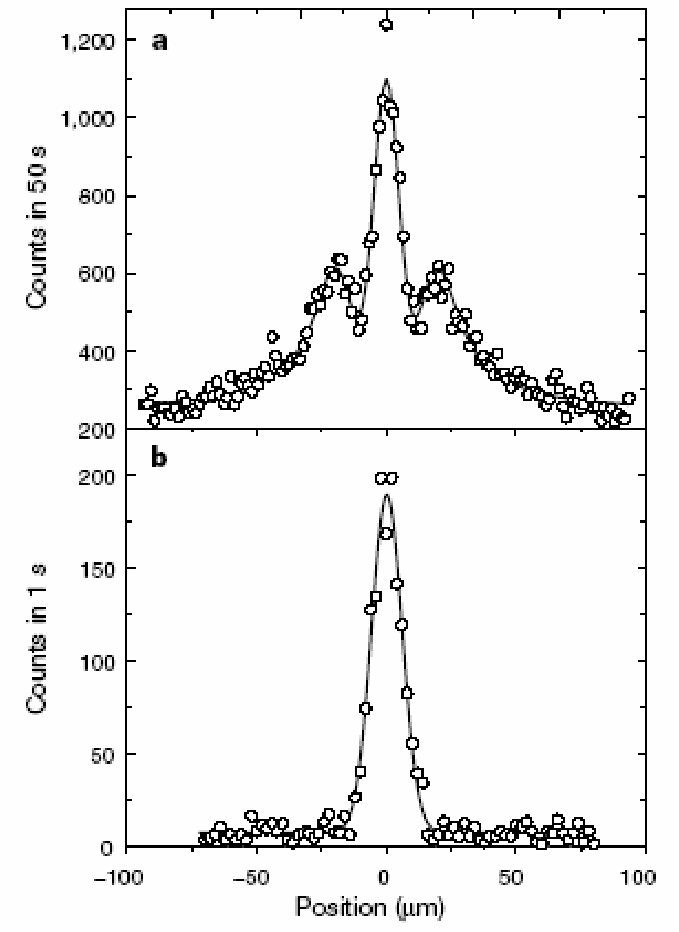
\includegraphics[width=0.55\textwidth]{Pictures/Resultat.PNG}
\end{center}
\caption{\textit{Résultats. Source: [Nature \textbf{401} (2000) 691].}}
\end{figure}
\newpage
Depuis lors, cette expérience a été répétée avec d'autres molécules plus complexes, notamment le $C_{70}$, la tetraphénylporphyrine (TPP) $C_{44} H_{30} N_4$ ou encore le fluorofullerène $C_{60} F_{48}$.

\paragraph{Exercice 4} \textit{La relation d'incertitude de Heisenberg}.
\begin{enumerate}
\item Nous désirons illustrer ici le fait que les propriétés ondulatoires de la matière ne sont pas pertinentes pour décrire le monde macroscopique. Considérons une particule d'un micromètre de diamètre, et de masse $m = 10^{-15}\, kg$. Calculez la longueur d'onde de De Broglie correspondant à cette particule si celle-ci se meut à une vitesse moyenne de $1\, mm /s$. Commentaires ?
\item Soit un virus d'une taille de $10 \, \mathring{A}$. Supposons que sa densité soit celle de l'eau, et qu'il soit confiné dans une région de largeur caractéristique approximativement égale à son diamètre moyen. Quelle est la vitesse minimale de ce virus ?
\end{enumerate}